\pdfminorversion 7
\pdfobjcompresslevel 3

\documentclass[a4paper]{article}
\special{papersize=210mm,297mm}
\usepackage[utf8]{inputenc}
\usepackage[T1]{fontenc}
\usepackage{cite}
\usepackage[francais]{babel}
\usepackage[bookmarks=false,colorlinks,linkcolor=blue]{hyperref}
\usepackage[top=3cm,bottom=2cm,left=3cm,right=2cm]{geometry}
\usepackage{graphicx}
\usepackage{subfig}
\usepackage{eso-pic}
\usepackage{array}
\usepackage{color}
\usepackage{url}
\usepackage{listings}
\usepackage{eurosym}
\usepackage{url}
\usepackage{textcomp}
\usepackage{fancyhdr} 
\usepackage{tikz}
\usetikzlibrary{automata,positioning}
\usepackage[french]{algorithm2e}

\definecolor{lightgray}{gray}{0.9}

\title{Rapport de projet de PPAR}
\author{Rémy \textsc{El-Sibaie Besognet} -- Roven \textsc{Gabriel}}

\newcommand{\HRule}{\rule{\linewidth}{0.5mm}}


\begin{document}

\maketitle


\section{Introduction}

L'algorithme de Jacobi est une des méthodes de résolution de systèmes
linéaires à diagonales dominantes. C'est le genre de problème qui
fourmille dans l'écosystème de la programmation parallèle de part la
grande quantité de calculs à éffectuer et sa potentielle simplicié à
être exploité par de multiples processeurs.

Le but de ce projet de PPAR est d'analyser une version séquentielle de
la méthode de Jacobi en C, et d'en fournir une version parallèle à
différents niveaux, notemment multi-processus, puis
multi-threading. On utilisera les bibliothèques OpenMPI et OpenMP pour
ce faire. On se posera la question des performancs en fonction des
communications éffectuées et du nombre de processeurs en comparant les
différentes approches. La première, plus naïve, implémentera une
architecture plus simple. On affine cette dernière au fur et à mesure
de l'exercice.

\section{Implémentation} 

\subsection{Condition de terminaison en parallèle}

La méthode de Jacobi correspond à une recherche de point fixe. On
itère jusqu'à ce que le résultat ne change plus. La condition d'arrêt
séquentielle est que la différence entre le résultat de l'itération
précédente et celui de l'opération courante soit inférieure à un
$\epsilon$ petit, c'est à dire la convergence.

Dans le cas parallèle la condition d'arrêt ne change pas, mais elle
doit être calculée sur tout les processus en même temps, qui auront,
le même résultat une fois celui-ci mit en commun.

\subsection{Implémentation naïve}

L'approche la plus naïve pour implémenter Jacobi à l'aide de la
méthode de Jacobi est d'utiliser une procédure de communication
collective : \texttt{MPI\_Allgather}. Celle-ci est faite pour
servir notre intérêt : réunir en un seul éléments des éléments d'un
même résultat, comme indiqué figure~\ref{allgather}. Le but est de
découper la matrice en $P$ (nombre de processus) blocs de lignes et de
réunir les résultats.


\begin{figure}
\centering
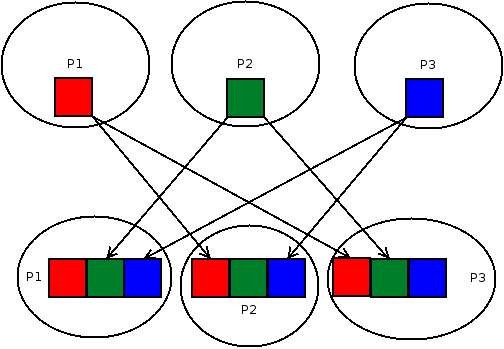
\includegraphics[scale=0.4]{allgather.png}
\caption{\label{allgather}Comportement du MPI\_Allgather}
\end{figure}

On doit s'arranger pour diviser chaque itération sur les différents
processus. La subtilité, dans cette approche est de ne pas oublier la
position de la diagonale dans le bloc de ligne du processus courant.
On admettra simplement, dans chaque processus, que les éléments de la
diagonale ne se trouvent pas en $A[i * h + i] $. Si $hlocal$ est la
hauteur de bloc, on aura une diagonale en $A[i * h + i + hlocal *
rang]$ qui correspond à un décalage de la diagonale de $rang$ fois la
hauteur de bloc.
Le pseudo code est détaillé dans l'algorithme~\ref{jacnaif}

\begin{algorithm}[H]
 \SetLine % For v3.9
 %\SetAlgoLined % For previous releases [?]
 \Repeter{non convergence et iter < maxIter}{
 iter $\leftarrow$ iter + 1\;
 
    \Pour{i = 0 à hlocal}{
     \Pour{j = 0 à n} {
             \dots 
        }
        \dots
      }

    
    MPI\_Allgather(xNew, hlocal, xPrev, hlocal)\;

    }
 
 \caption{\label{jacnaif}Jacobi avec \texttt{MPI\_Allgather}}
\end{algorithm}


Cette méthode a l'avantage d'être très simple à la fois à mettre
en \oe uvre et à relire. Mais elle a un énorme problème de
performaces. A chaque itération on a $n - 1$ communications par
processus et donc au total une complexité en messages de $n*(n - 1)$,
soit $O(n^2)$. Ceci n'est pas souhaitable, car la solution sera
inutilisable si le nombre de processus grandit trop (perte en
efficacité). C'est pour cette raison que nous nous dirigeons vers une
autre architecture.


\subsection{Implémentation en anneau}

\subsection{Algorithmes d'initialisation et de vérification}

\section{Optimisations}

\subsection{Recouvrement des communications par le calcul}

\subsection{Parallèlisation hybride : MPI + OpenMP}

\section{Conclusion}

\end{document}

# Local Variables:
# compile-command: "rubber -d rapport.tex"
# End:
